\documentclass[uplatex]{jsarticle}
\usepackage[dvipdfmx]{graphicx}
\begin{document}
\begin{flushright}
  鈴木理也
\end{flushright}

\setcounter{section}{1}
Chapter2
\section{二階線形微分方程式}

\subsection{Problem set 2.4}
\large
1.初期値問題(4)${y_0},{v_0}$を初期値とした周期運動を見つける。
  ${\omega_0}={\pi},{y_0}=1$として、
  $$ my'' + ky =0 $$

  $$ {\lambda}^2 +\frac{k}{m} = 0 \leftrightarrow {\lambda} = \pm i {\sqrt{\frac{k}{m}}}$$ 
  ${\omega_0}={\sqrt{\frac{k}{m}}}$とすると

  $$ y(t) = A cos({\omega_0}t) + B sin({\omega_0}t) $$

${y_0}$から始まり${v_0}$が初期速度なので
$$ y_0 = A cos(0 * \pi) + B sin(0* \pi)$$
$$ y_0= A = 1$$


微分して


$$ y'(t) = -{\omega_0} A sin({\omega_0}t) + {\omega_0} B cos({\omega_0}t) $$
$$ v_0 = -{\omega_0}A sin 0 + {\omega_0}B cos 0 $$
$$ v_0= -{\omega_0}A*0 + {\omega_0}B*1 $$
$$ v_0 = {\omega_0}B $$
$$ B = \frac{v_0}{\omega_0} $$
A,Bを入れると、こうなる。
$$ y(t) = cos({\omega_0}t) + \frac{v_0}{\omega_0} sin({\omega_0}t) $$
式の$v_0$を0,負、正とするとグラフはこうなる。


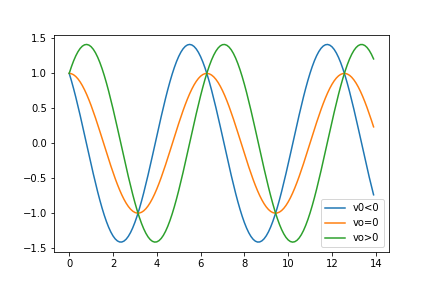
\includegraphics{./hertz.png}



2. 重さ20nt、バネを2cm伸ばした。調和振動と周期。
$$ W = 0.02k $$

$$ k = \frac{W}{0.02}= \frac{20}{0.02} = 1000kg/sec^2 $$

$$ m = \frac{W}{g}= \frac{20}{9.8} \approx 2.04(kg) $$

$$ f = \frac{\omega_0}{2\pi} = \frac{\sqrt{\frac{k}{m}}}{2\pi} \frac {\sqrt{\frac{1000}{2.4}}}{2\pi} = \frac{\sqrt{490.19}}{2\pi} \approx 3.52(Hz)$$


3. 重さを2倍にしたときと、バネを二倍にしたとき



*重さが2倍の場合
$$ f = \frac{\omega}{2\pi} $$
$$ \omega = \sqrt{\frac{k}{m}}$$
$$ \omega_1 =\sqrt{\frac{k}{2m}} = \frac{1}{\sqrt{2}}* \sqrt{\frac{ k}{m}}= \frac{1}{\sqrt{2}}* \omega$$
$$ f_1 = \frac{\omega_1}{2\pi}= \frac{1}{\sqrt{2}}*f $$
$ \frac{1}{\sqrt{2}}$ 周期が遅くなる



*バネを二倍にした場合
$$ \omega_1 =\sqrt{\frac{2k}{m}} = \sqrt{2} \omega$$
$$ f_1 = \frac{\omega_1}{2\pi}= \sqrt{2}f $$
$ \sqrt{2} $ 周期が早くなる。


4. いいえ
$$ \frac{k}{m} に関係しないから$$
5. バネをいろいろ

$$ f = \frac{\omega}{2\pi} $$

1, $ f = \frac{\sqrt{\frac{20}{5}}}{2\pi} $
$$ f= \frac{2}{2\pi} $$
$$ f = \frac{1}{\pi}$$
$$ \approx {0.318}Hz $$

2, $ f = \frac{\sqrt{\frac{45}{5}}}{2\pi} $
$$ f=\frac{3}{2\pi}$$
$$ \approx{0.477}Hz $$

3, $ f = \frac{\sqrt{\frac{k_1+k_2}{m}}}{2\pi} $
$$ f = \frac{\sqrt{\frac{20+45}{5}}}{2\pi} $$
$$ \approx{0.574}Hz$$

\end{document}
